\documentclass{article}

% Language setting
% Replace `english' with e.g. `spanish' to change the document language
\usepackage[english]{babel}

% Set page size and margins
% Replace `letterpaper' with `a4paper' for UK/EU standard size
\usepackage[letterpaper,top=2cm,bottom=2cm,left=3cm,right=3cm,marginparwidth=1.75cm]{geometry}

% Useful packages
\usepackage{amsmath}
\usepackage{amssymb}
\usepackage{graphicx}
\usepackage{bm}               % great math stuff
\usepackage{amsfonts}              % for blackboard bold, etc
\usepackage{amsthm}                % better theorem environments
\usepackage{amssymb}
\usepackage{mathtools}             %needed for normbg command
\usepackage{stackengine}
\usepackage[colorlinks=true, allcolors=blue]{hyperref}

% \theoremstyle{definition}
\theoremstyle{definition}

\newtheorem{definition}{Definition}[section]
\newtheorem{theorem}{Theorem}[section]
\newtheorem{lemma}[theorem]{Lemma}
\newtheorem{proposition}[theorem]{Proposition}
\newtheorem{corollary}[theorem]{Corollary}
\newtheorem*{theorem*}{Theorem}


% \newtheorem{definition}[theorem]{Definition}
\newtheorem{remark}[theorem]{Remark}
\newtheorem{notation}[theorem]{Notation}
\newtheorem{question}[theorem]{Question}
\makeatletter
\newcommand{\cbigoplus}{\DOTSB\cbigoplus@\slimits@}
\newcommand{\cbigoplus@}{\mathop{\widehat{\bigoplus}}}
\newcommand{\tens}[1]{%
  \mathbin{\mathop{\otimes}\limits_{#1}}%
}
\makeatother
\title{A Generalization of Buckingham Pi}
%\title{Neural Net Aided Solutions to Post Collision Behavior of Yield-Stress Fluids}
\author{Jack R. Goldrick}

\begin{document}



\maketitle

\begin{abstract}
In the absence of governing equations, understanding the behavior of momentum in Yield-Stress Fluids (YSFs) can be rather difficult. These governing equations, such as a system of PDE's, are transformable to a non-unique non-dimensionalized space. A common method used is the Buckingham Pi Theorem which creates its famous pi-groups to accomplish the desired transformation. In 2015, TK Blackwell TK conducted an experiment to determine the post collision behavior of rheological fluids resulting in 5 regimes maps and a governing dimensionless variable that accurately describes the behavior. This study aims to develop a low resource neural net aided solution to identifying the behavior of the yield-stress fulids studied by Blackwell et al.

\end{abstract}

\begin{align*}
    \title{Notation} 
\end{align*}

\begin{description}
    \item[$(\mathbb{F}, \mathfrak{F})$] The Feature Space is the set of all measurable parameters with respect to some dynamical system $\mathfrak{F}$.  Often if the system is well known, we can short hand this to $\mathbb{F}$
\end{description}
%$(\mathbb{F}, \mathfrak{F})$ is the set of all measurable parameters with respect to $\mathfrak{F}$.  Often if the system is well known, we can short hand this to \mathbb{F}


\section{Introduction}

\subsection{Background}

Yield-stress fluids are a vital resource in Industrial Engineering. These fluids are used in areas relating to agriculture and food processing, feedback control and safety systems, along with manufacturing [I Think I need to reference this].  Many of these processes can be aided by having real-time data driven methods that can provide an optimized and low-cost feedback control platform. Computational Fluid Dynamics (CFD) is extremely resource intensive and cannot be reliably used for real-time control. For reference, a simple T-Junction pipe flow solution from my undergrad took about 1.5hrs to fully render results on a GPU architecture.  This glaring inefficiency overtly exceeds an acceptable time-to-compute (TTC) and must be optimized to handle scaling required by Industry. Many industry applications may involve fluid droplets contacting wet and/or dry surfaces and this simple difference can have dramatic consequences. To describe this difference, Blackwell [TK TK] denotes a situation where the parameter, surface hydrophobicity, may hold no predictive value, but the impact surface is completely wet prior to collision. This surface condition increases the minimum dimension of a model's parameter space. In the case described by Blackwell, the added parameter (dimension) is the thickness of the pre-coating layer which has high predictive value in models used to predict the collision behaviors of the described situation. So in the absence of governing equations how is one possibly supposed to arrive at the conclusion described by Blackwell? 

\subsection{Buckingham Pi}
    
Since its discovery in the late 1800s as a generalization to the Rayleigh Method, the Buckingham Pi Theorem has become a quintessential tool used in dimensional analysis.  The Buckingham Pi theorem states there exists a set of dimensionless quantities, known as $\pi$-groups, that span the full dimensionless solution space.  A probabilistic corollary to the theorem states there must exist some function that projects a dataset to a lower dimensional space without a significant increase in the predictive error on the dataset [TK I think this needs a cite? it is heavily paraphrase from blackwell].  Blackwell's absence of governing equations makes Buckingham Pi the perfect analytical tool to gain a glimpse into the dynamics of momentum in Yield-Stress Fluids.  It is important to note that may be fruitless to fully map all parameters, $p \in \mathbb{P}$, that dictate the full dynamics of a system.  This fruitless overtone is a consequence of Buckingham Pi's one major pitfall: a set of $\pi$-groups derived from the solution is not unique.  Properties such as shear viscosity have been shown to be quite difficult to measure and can lead to a gap in necessary information for regression-based modeling, especially if the parameter has a high predictive value.  Machine learning algorithms can circumvent the need to understand the governing dynamics thus making algorithms like SINDy unnecessary in applications described by Blackwell. This philosophy will be later used to derive a new use case for Buckingham Pi with respect to machine learning applications.

\subsection{Machine Learning and Graphs}

Given the general behavior of YSFs, there are many computational complexities and accuracy issues that arise from linear algorithms trying to predict high dimensional non-linear phenomena of YSFs.  Certain machine learning algorithms have been shown to model well under these conditions and can provide the multi-class outputs needed to accurately model YSFs in the absence of a differential system.  Ideally, these algorithms should help find some map $f: \mathbb{P} \xrightarrow{} \mathbb{D}$ that maps every dimensional input parameter $\boldsymbol{p}\in \mathbb{P}$ to a classification category $\boldsymbol{d}\in \mathbb{D}$ such that error is minimized.  Decision Tree and Neural Net based algorithms are readily equipped to fit and evaluate these kinds of datasets since they are both variations of Directed Acylic Computational Graphs (DACGs).
%  This is a Direct Quote from my textbook. How should this be cited?
\begin{definition}[Directed Acyclic Computational Graph]
    A directed acyclic computational graph contains nodes, so that each node is 
    associated with a variable. A set of directed edges connect nodes, which indicate functional relationships among nodes. Edges might be associated with learnable parameters. A variable in a node is either fixed externally (for input nodes with no incoming edges), or it is computed as a function of the variables in the tail ends of edges incoming into the node and the learnable parameters on the incoming edges.
\end{definition}

Most DACGs contain three types of nodes/layers: input, output, and hidden.  The I/O nodes and layers are responsible for determining the dimension of the parameter and solution space.  Whereas, the hidden layers contain and process intermediate values to find distinguishing features of each $\boldsymbol{p}\in \mathbb{P}$.  These graphs use functions either defined by the user in the case of Neural Networks or other metrics like those used in Decision Trees.  These functions are not constrained by linearity and often times are used non-linearly to transform features such that models can predict a high dimensional and nonlinear set of data similar to Blackwell.  





\subsubsection{Decision Trees and Random Forests}

A Decision Tree can represent any map $f$ that is piecewise-constant on non-overlapping
regions of a feature space. A Decision Tree will define these non-overlapping regions using decision and leaf nodes.  Decision nodes represent some metric for partitioning the data, like p-norm of a vector must be positive.  A leaf node $l$, an edge-less node, represent a decision function $\mathcal{S}_l \subseteq \mathbb{P}$ in the feature space. The leaf nodes in the context of Blackwell's Data are the classification categories: the unique elements of $f(\mathbb{P})$.  Generally, Decision Trees are comprised of these nodes connected by unweighted directed edges giving step-by-step instructions on computing the function value $f(\boldsymbol{p})$ given the features of each $\boldsymbol{p}\in \mathbb{P}$.  Simply put, these models begin by feeding each $\boldsymbol{p}$ through a root node and outputting each $\boldsymbol{d}$ at a leaf node.  This architectures allows the final shape of a decision tree to be highly complex allowing for extensive nonlinear modeling of a hypothesis space.  Decision tree methods use as a hypothesis space the set of all hypotheses which represented by some collection of decision trees.  Thus, large decision trees can represent complicated partitions that map any given labeled dataset.  A random forest expands on this by fitting a number of decision tree classifiers on various sub-samples of the dataset and uses averaging to improve the predictive accuracy and control over-fitting. These methods search for a decision trees such that the corresponding hypothesis has minimum average loss on some labeled training data [TK Mostly quoted from keras documentation].  Therefore, a sufficiently large decision tree or deep forests can obtain the ideal map $f$ that best minimizes error for any given non-linear map.  [TK This is fairly heavily paraphrased from my textbook, how should I cite?]




% tree is constant over the regions Rm , such that h(x) = h m for all x ∈ Rm and some
% fixed number h m ∈ R.


\subsubsection{Neural Networks and Deep Learning}

DACGs have insurmountable predictive capabilities when designed as Neural Networks.  Neural networks are one of the most prevalent applications of a multi-layer DACG and achieve their high predictability by combining multiple layers of nodes (neurons).  A network's neurons are arranged layer-wise, such that all neurons in the $i$\textsuperscript{th} layer are connected to the neurons in the $i$\textsuperscript{th}$+1$ layer. The layer-wise architecture of neurons constructs the input space such that the variables in each layer can be written as a vector function of the variables in the previous layer.  Activation functions can be used at each hidden layer but are not added to the input layer, however, given multi-class classification problems, the output layer almost always utilizes the activation function: softmax.  This vast customizablility to a network's architecture is what practically gives a network its capabilities to model high dimensional and non-linear datasets.  


\begin{figure}
\centering
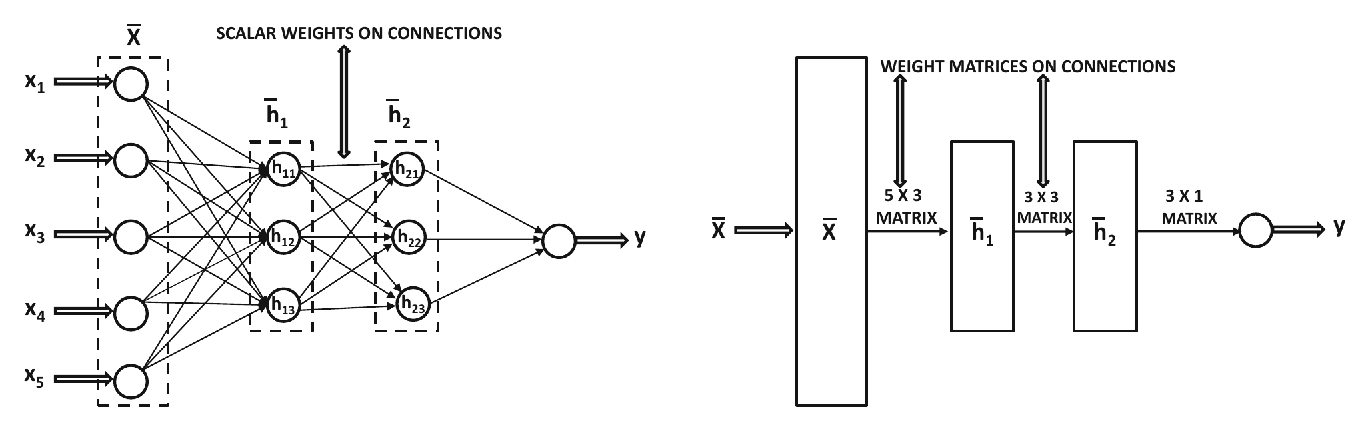
\includegraphics[width=1\linewidth]{pics/nn_graphs.png}
\caption{\label{fig:nng}This is from my textbook, I am making my own. This is just a placeholder}
\end{figure}


Figure 1 demonstrates two common diagrams used to represent a multi-layer neural network.  In this
example, the network contains three layers in addition to the input layer.  Neural Networks are the abstract application of Tensor objects and part b of Figure 1 shows how Neural Networks take that form as matrices.  For example, consider the first hidden layer with output values $ h_{11}, ..., h_{1 \alpha}, \forall \alpha \in \mathbb{N} $ that are computed as a function of the inputs $x_1, ..., x_{\beta}, \forall \beta \in \mathbb{N}$.  

% Talk about matricies and shit here to finish out the theory.


Since Tensors have a wonderful ability to perform calculus and algebra operations, they have been used extensively to define Neural Networks. 





%add activation functions to become better approximators to almost all class of functions. 












% Two popular choices for the activation function used within artificial neural net-
% works are the sigmoid function f (z) = 1
% 1+exp(−z) or the deep net f (z) = max{0, z}.
% Artificial neural networks using many, say 10, hidden layers, is often referred to as a
% deep net. ML methods using hypothesis spaces obtained from deep nets are known
% as deep learning methods [7].
% Remarkably,usingsomesimplenon-linearactivationfunction f (z) asthebuilding
% block for artificial neural networks allows us to represent an extremely large class of
% predictor maps h(w) : Rn → R. The hypothesis space generated by a given artificial
% neural network structure, i.e., the set of all predictor maps which can be implemented
% by a given artificial neural network and suitable weights w, tends to be much larger
% than the hypothesis space (2.4) of linear predictors using weight vectors w of the
% same length [7, Chap. 6.4.1.]. It can be shown that an artificial neural network with
% only one single (but arbitrarily large) hidden layer can approximate any given map
% h : X→ Y= Rto any desired accuracy [8]. However, a key insight which underlies
% many deep learning methods is that using several layers with few neurons, instead
% of one single layer containing many neurons, is computationally favourable [9].









 % \newline
 % \newline
 % \newline
 % \newline
 % \newline

% AAAAAAAAAAAAAAAAAAAAAAAAAAAAAAAAAAAAAAAAAAAA \newline
% AAAAAAAAAAAAAAAAAAAAAAAAAAAAAAAAAAAAAAAAAAAA \newline
% AAAAAAAAAAAAAAAAAAAAAAAAAAAAAAAAAAAAAAAAAAAA \newline
% AAAAAAAAAAAAAAAAAAAAAAAAAAAAAAAAAAAAAAAAAAAA \newline
% AAAAAAAAAAAAAAAAAAAAAAAAAAAAAAAAAAAAAAAAAAAA \newline
% AAAHHHHHHHHHHHHHHHHHHHHHHHHHHHHHHHHHHHHHHHHH \newline
% HHHHHHHHHHHHHHHHHHHHHHHHHHHHHHHH




% , potentially restrictive, conditions and even outperform regressors by a factor of 1.5. 

 % of Blackwell's dataset: multidimensional inputs with multiple qualitative outputs.

% leading to many issues with creating accurate models of behavior [TK I think this needs a cite? it is heavily paraphrase from blackwell].     

% TK TK Do i need to tek a sample of the buckingham pi procedure?

% I do not know what else would be pertinent?






% There are many computational complexities and accuracy issues arise from linear machines trying to predict high dimensional non-linear phenomena.



\section{Methodology}


% There was an issue with Bucki-Net that was ever present before the data was manipulated: What if Bucki-Net does not pick Blackwell's dimensionless variable as a $\pi$-group? Or worse: What if the data-driven output function is only surjective? 

% \subsection{Data Manipulation and Processing}
% Yes there is a GenZ double entandre in this section.  I did not plan it but its staying now :)
Python is by far one of the best languages for data analysis given the large open-source libraries that can be imported.  Blackwell's Data was imported with pandas and numPy, while the modeles were built with Keras and scikit learn libraries with Tensorflow and PyTorch in the backend when needed.  Every *Prep.ipynb was used, as the name implies, to prep the data for all these models to cook with.  Important steps taken to ensure proper encoding including using the one-hot schemes on the output class and scaling of the input dataset.  Unscaled datasets drastically reduce almost every model's performance; thankfully, Sci-Kit Learn and Keras has a data transformer prepackaged.  The Sci-kit Learn library has prepackaged many Decision Models that can fit a wide variety of datasets. The beauty of this packages is it's plug and play functionality that requires a few argument's to run.  Keras is another easy to use library that has a heavily customizable feed-forward neural network package. For those readers curious about the code and engineering side of the methodolody, I refer them to the project's repository: computationalWaterBending on my github.  The following methodology will focus on the mathematical abstraction and generalization of Buckingham Pi called the Golden Pi Theorem.  This theorem strips Buckingham Pi of its notions of functional relationships and replace it with a foundation of Measure Theory to create it's Pi Groups.
 % Or worse: What if the data-driven output function is only surjective? 
\subsection{Dynamical Measure Spaces and The Golden Pi Theory}
The goal with Buckingham Pi was to be used as the inputs to a machine learning model. However, There was an issue with Bucki-Net that was ever present before the data was manipulated: What if Bucki-Net does not pick Blackwell's dimensionless variable as a $\pi$-group?  Well, that is exactly what happend and the proceeding subsection will dive into the methods used to create multiple dimensionless groups.  


\begin{theorem}
    
    $F = \{f_1, f_2, ..., f_n: n \in \mathbb{N}\} \subseteq{}$ is a collection of measurable parameters from a dynamical system $\mathfrak{F}$ if the following hold:
    \begin{enumerate}
        \item $F \subseteq (\mathbb{F}, \mathfrak{F})$

        \item $ f_n = f_m  \iff m = n, \ \forall n, m \in \mathbb{N}_{\leq |\mathbb{F}|}$ 
    \end{enumerate}
    
    % $(\mathbb{F}, \mathfrak{F})$ is the set of all measurable parameters with respect to $\mathfrak{F}$.  Often if the system is well known, we can short hand this to \mathbb{F}
    
    
    %Thus, let $ \mathbb{F} \subseteq \mathbb{R}^{n}$ be measurable space of elements that belong to our feature space. These measurable elements are any measurable property of a system like flow stress and thus we have  
    
    

\end{theorem}

\begin{definition} 
    Following from Theorem 2.1, let $ \Psi: \mathbb{F} \mapsto \mathbb{P} $ be the function that maps the feature space to the parameter space. Thus, $\mathbb{P} \subseteq \mathbb{R}^{n}$ from $F$ is defined as \newline
    \[ \mathbb{P} =  \Psi(\mathbb{F}) :=
    \bigoplus_{i \in \mathfrak{I}_n}f_i, \quad \forall f \in F    \]

\end{definition} % I need to tweak slightly 

\begin{definition}
    Once the parameter space has been constructed using Definition 2.1, the following set of functions, $\Gamma = \{ \gamma_i | \ \forall i \in \mathfrak{I}_{E},  \gamma_i: \mathbb{P} \mapsto P \subseteq \mathbb{R}^{m \  \times \ n} \}$  pairs the parameter space to each $_i \in E$, where $E$ is the set of all experiments. Given the nature of the pairing, we can define this set with the outer product as follows: 
        $$ P_{ij} =   \gamma_i (p_j) = \Gamma \otimes \mathbb{P} $$
\end{definition} % \Gamma_i(\mathbb{P}_j) =

\begin{definition} Let $\Omega: \mathbb{F} \mapsto \mathbb{R}^{d} $ be a function that maps a measurable quantity, $f_n$, to a vector containing the powers of $d$ basic reference dimensions like mass, length and time.  For example, the units of a force are Newtons and in terms of mass, length and time we have $[Force]  = ML/T^{2}$. Thus, $$\Omega(Force) = [1, 1, - 2]^{T}$$ 

    % I think this needs a cite
\end{definition}

\begin{definition}
    Let $\phi: \Pi \mapsto \mathbb{R}^{n}$ be a function that maps a dimensionless group to a vector that corresponds to the powers of each $f_n\in F$ such that 
    $$\phi(\pi_{j}) = [\Phi_{1j} , \Phi_{2j} , . . . , \Phi_{nj} ]^{T}, \quad \forall n \in \mathbb{N}_{\leq |\mathbb{F}|} \  \land \ j \leq n - d  $$
\end{definition} % I think this definitely needs a cite

\begin{definition}
    Let $T : F \mapsto U$ be the function that maps the feature space to the units matrix, $U$, of the Buckingham Pi Theorem. The units matrix is constructed with the direct sum along mode two as follows:

      $$ U =  T (\mathbb{F}) = \bigoplus_{i \in \mathfrak{I}_n} \Omega(f_i), \quad \forall f \in F$$
\end{definition}

\begin{lemma}
    The use of definitions 2.4 and 2.5 to construct the Buckingham Pi Theorem will guarantee $$\phi(\pi_j) \in \ker(U), \quad \forall \ j \leq n - d$$ 
\end{lemma}

\begin{definition}
    The Pi-Groups power matrix, $\boldsymbol{\Phi}$, is given by the following function , $\Phi: \Pi \mapsto \mathbb{R}^{n \times (n - d)}$, as a direct sum along mode two 


    $$ \boldsymbol{\Phi} =  \Phi(\Pi) = \bigoplus_{j \in \mathfrak{I}_\Pi} \phi(\pi_j), \quad \forall \ j \leq n - d$$
\end{definition}


\begin{definition}
    Once $\boldsymbol{\Phi}$ has been constructed from Lemma 2.2 and definition 2.6, a function $\Theta : P \mapsto \Pi$ maps the dataset P to it's dimensionless representation as follows

    $$ \Pi = \exp(\log(P) \boldsymbol{\Phi})$$
\end{definition}

\section{Results}

\subsection{General Model Comparison}

The two models with the best overall performance were Neural Networks and Gradient Boosted Random Forests (GBRFs).  It is likely that with a proper means of optimization that Neural Networks would reign supreme over Decision Tree methods.  The architecture of both networks  and forests seemed to be tied to the basis chosen.  However, after some tweaking the models were able to regain almost all their accuracy lost from the basis change.  Consistency was a different story for both of the top performers;  GBRFs  seemed to excel in consistency, rarely faltering to a degree that the maximum accuracy was the average accuracy.  Whereas,  depending on the architecture, techniques such as  orthogonal-regularization in the linear layers and dynamic sparsity enforcement on linear layers tightened the spread against testing accuracy.  In Addition, hyperbolic and scaled-sigmoid (silu) activation functions seemed to tighten the spread of the pi-groups as well.  In contrast, within the noseWaterTree.ipynb, it can be seen that some form of a leaking rectilinear activation function was important to ensure a Neural Network's peak accuracy.   Upon further inspection of the Nose Water Tree Notebook File,  it would be reasonable for some confusion to arise when trying to understand the similarities in network architecture and accuracy tier, as it is still not absolutely clear why this occurred.  It should also be noted that probablistic metrics and loss functions had the most significant role in decreasing the spread of testing accuracy.  Over-parameterization was a precarious obstacle  that plagued many architectures.  


\subsection{Non-Dimensionalization and Physical Meaningfulness}

The use of dimensioned vs nondimensioned data played a significant role in overall model performance on both training and test sets.   Without the use of Hyperparamters, almost all models seemed to struggle  making sense of the dimensioned data.  Decision tree models had the highest degree of variability causing a wide range of accuracy values on both the test and training sets.   There were some pi-basis that obliterated the structure within the dataset causing accuracy values to drop below 50\%.   These degenerative basis sets were typically very odd dimensionless numbers that did not seem to have any use in the field of rheology.   To contrast with a positive result, once Blackwell's Number and length scale was given to the models as inputs,  all models  saw significantly increased performance allowing some Forest Models to consistently outperform the rest at about 93\% accuracy.   It is important to note that no matter the basis chosen, in general, an unguided nondimensionalization, using the methodology in section 2, will increase most model's performance by a minimum of 10\% when compared to the same model on dimensioned data.   Thus, with more experimentation on other systems, it wold be more than reasonable to conclude that section 2's technique is an easy and cheap way to improve almost any model's performance.  However, the technique, so far, does not have a means to analyze the concept of physical meaningfulness.    Bakarji  defined physical meaningfulness as the dimensionless group’s ability to simplify an equation in relevant regimes and provide a scaling that collapses the input-output solution space to a lower dimension [TK CITE BAK TK].   Blackwell substantiated this definition when talking about the dynamics of their system which lead them to determine their dimensionless number should include flow, inertial forces, diameter and thickness.  These results seem to imply some underlying mathematical structure that governs physical meaningfulness or the system, but more experimentation is needed to help support a proof of this concept.   

%Currently, it seems there are isometries and/or isomorphisms between pi-groups and some algebras.   These structural similarities may be key to understanding the generalization.  

The Golden Pi Methodology yielded five pi groups that had some interesting properties and potentially noteworthy definitions that could reveal .  First key result was Blackwell's Numbers and Scales were found to be in the span of both representations of the space spanned by the gPi Groups.  The indices of the vector $\boldsymbol{x}$ represent the coefficients responsible for creating the linear combination of gPi groups that create any new dimensionless numbers such as Blackwell's.  This vector $\boldsymbol{x}$ satisfies the equation: $\boldsymbol{\pi}_{\boldsymbol{x}} = \boldsymbol{\Phi} \boldsymbol{x} $.  Assuming there was some way to target Blackwell's Number with some algorithm, one simply needs to solve for $\boldsymbol{x}$ via the least squares regression algorithm return a function that will encode the data to be represented with Blackwell's Numbers and Scales.  Given this relation, it is likely the image of $\boldsymbol{\Phi}$ contains both physically meaningful and frivolous dimensionless quantities.  Neural Networks seemed to back this up as there The function $\Phi$  on the Pi-Space, $\Pi$, appears to isometrically and isomorphically map $\Pi \subseteq \mathbb{R}  $ to a subset of $ \mathbb{R}^{n \times (n-d)}$ but has no inherit optimization that can steer it towards a better basis.  If it is the case that there are isometric and isomorphic mappings between all these spaces, then it is likely that the underlying behavior of Dynamical Measure Spaces can be well understood in the absence of governing equations.  


%from scipy.optimize import minimize
%import numpy as np
%
%# Define your matrix A and constraint function (for example, b = Ax)
%A = np.array([[1, 2], [3, 4], [5, 6]])
%def constraint(x):
%return A @ x - b
%
%# Define your relevance function f(b)
%def f(b):
%return np.sum(np.abs(b))  # Example: sum of absolute values
%
%# Define the objective function with L2 regularization
%def objective(x):
%b = A @ x
%return -f(b) + lambda_ * np.linalg.norm(b)**2
%
%# Initial guess for x
%x0 = np.zeros(A.shape[1])
%
%# Regularization parameter
%lambda_ = 1.0
%
%# Solve the optimization problem
%result = minimize(objective, x0)
%
%# Optimal x
%x_optimal = result.x
%b_optimal = A @ x_optimal
%




%The models used to evaluate Blackwell's data seemed sensitive to the pi basis used; this sensitivity seems concurrent that there are more physically meaningful numbers that best minimize loss as discussed by Bakarji. 


%This result was also not completely unsurprising, since,  Blackwell and Bakarji both spoke of the importance of physical meaningfulness in the construction  of their analysis.   

%\subsection{Algebraic Behavior and Matrix Analysis} 



  

\subsection{Blackwell's Pi Groups vs. Golden Pi Groups}

On a 80/20 train-test split, a basic logistic regression had its average accuracy match it's maximum accuracy of 86.54\% compared to the dimensional accuracy of 67.31\%.   Decision Trees and Random Forests had an incredible show of force at 92.31\%  where again the maximum matches the average.  GBRFs performed slightly better,  classifying one or two more instances correctly with the same near perfect consistency.   Unfortunately, the Golden Pi Theorem did not fair well against the Blackwell's Numbers and Length Scales combined with the Golden Pi's methodology on a subset of measurable parameters.  When the nondimensionilzation techniques were compared with these models, Blackwell's Set was by far the best transformation for the dataset in terms of peak performance metrics only.   However, Neural Networks had a much different reaction to the various non-dimensional sets.


Neural Networks with the high accuracy peaked at 96.15\% with an average accuracy as high as 94\% but more often than not the average was about 83-89\%.  The most consistent high running average was about 92\% which is incredible considering that translates to less than or equal to five wrong depending on the split.  The golden pi groups  also outperformed their dimensional counterparts by a minimum of 10\% on every model.  Interestingly, the Golden Pi Groups lacked behind the peaks of Blackwell's numbers by a maximum of 20\% at times  but on average lacked by a significantly smaller margin of 6\%.  
 Given that all of Blackwell's Numbers, $\pi_{B_{j}} $, are in the span of Img($\boldsymbol{\Phi}$), it is possible that there is some geometric or algebraic link to the pi-groups that can exploited from the fundamental Matrix Subspaces.


%However,  due to time limitations, a similar high performance was not discovered for the Golden Pi Groups.  Even though a high performance model was not found, it is unlikely this is a result of the methodology but rather the concept of physical meaningfulness. 






% \subsubsection{Random Forests}


% \subsubsection{Gradient Boosted Forests}

% \subsection{Neural Networks}



\section{Discussion \& Conclusion}

The unguided Kernel Transformation was a significant improvement for all models tested and was shown to have radical improvements on a subset of the models.  While successful, Blackwell's Numbers and Scales were far better estimators and it is unclear how to guide this method toward the proper numbers.  Given the behavior of these network models, it is more likely that this method shifts the burden of optimization to the model's architecture.  This is the new hypothesis for testing in phase two of this study.  




%Blackwell's Numbers and Scales are found to be in the span of Img($\boldsymbol{\Phi}$)  and thus its solution is unique to the system.  



% if their number exist with the span of Img($\boldsymbol{\Phi}$) there exists a perf
%\subsection{How to add Citations and a References List}
%
%You can simply upload a \verb|.bib| file containing your BibTeX entries, created with a tool such as JabRef. You can then cite entries from it, like this: \cite{greenwade93}. Just remember to specify a bibliography style, as well as the filename of the \verb|.bib|. You can find a \href{https://www.overleaf.com/help/97-how-to-include-a-bibliography-using-bibtex}{video tutorial here} to learn more about BibTeX.
%
%If you have an \href{https://www.overleaf.com/user/subscription/plans}{upgraded account}, you can also import your Mendeley or Zotero library directly as a \verb|.bib| file, via the upload menu in the file-tree.
%
%\subsection{Good luck!}
%
%We hope you find Overleaf useful, and do take a look at our \href{https://www.overleaf.com/learn}{help library} for more tutorials and user guides! Please also let us know if you have any feedback using the Contact Us link at the bottom of the Overleaf menu --- or use the contact form at \url{https://www.overleaf.com/contact}.

\bibliographystyle{alpha}
\bibliography{sample}

\end{document}\\
